\subsection{The seven computations of the composition product}

Let M, M', and M'' be three left A-modules, \(a : R \to M\) , \(a' : R' \to M'\) and \(a'' : R'' \to M''\) projective resolutions, \(c : M \to E\) , \(c' : M' \to E'\) and \(c'' : M'' \to E''\) injective resolutions. It follows from X, p.~100, th. 1 and p.~103, prop. 2, that the diagram:

\[
\begin{array}{c} \mathrm{H} (\operatorname{Homgr} _ {A} (M, E ^ {\prime})) \xrightarrow {} \mathrm{H} (\operatorname{Homgr} _ {A} (R, E ^ {\prime})) \xrightarrow {} \mathrm{H} (\operatorname{Homgr} _ {A} (R, M ^ {\prime})) \\ \uparrow \quad \xrightarrow {\varphi (M , E ^ {\prime})} \quad \downarrow \varphi (\mathbf {R}, E ^ {\prime}) \quad \uparrow \\ \mathrm{H} (\operatorname{Homgr} _ {A} (E, E ^ {\prime})) \xrightarrow {\varphi (E , E ^ {\prime})} \operatorname{Ext} _ {A} (M, M ^ {\prime}) \xleftarrow {\varphi (R , R ^ {\prime})} \mathrm{H} (\operatorname{Homgr} _ {A} (R, R ^ {\prime})) \end{array}
\]

where the unlabeled arrows are canonically deduced from \(c\) , \(a\) , \(c'\) , \(a'\) , is commutative, and that all the arrows are isomorphisms, which gives five descriptions of \(\mathrm{Ext}_{\mathbf{A}}(\mathbf{M}, \mathbf{M}')\) . One obtains likewise five descriptions of \(\mathrm{Ext}_{\mathbf{A}}(\mathbf{M}', \mathbf{M}'')\) , and as many of \(\mathrm{Ext}_{\mathbf{A}}(\mathbf{M}, \mathbf{M}'')\) .

Consider now the seven composition homomorphisms

\[
\mathrm{H} \left(\operatorname{Homgr} _ {\mathbf {A}} \left(\mathrm{C} ^ {\prime}, \mathrm{C} ^ {\prime \prime}\right)\right) \otimes_ {k} \mathrm{H} \left(\operatorname{Homgr} _ {\mathbf {A}} \left(\mathrm{C}, \mathrm{C} ^ {\prime}\right)\right)\rightarrow \mathrm{H} \left(\operatorname{Homgr} _ {\mathbf {A}} \left(\mathrm{C}, \mathrm{C} ^ {\prime \prime}\right)\right),
\]

where one takes successively for (C, C', C'') the seven triples (R, R', R''), (R, R', M''), (R, R', E''), (R, M', E''), (R, E', E''), (M, E', E''), (E, E', E'').

\pandocbounded{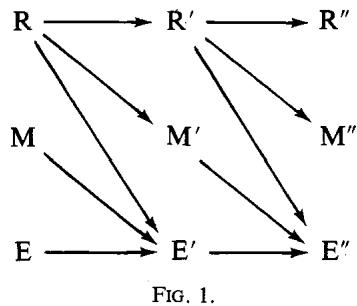
\includegraphics[keepaspectratio]{images/part001_66540ed3.jpg}}

Identifying H(Homgr \(_A\) (C, C')) with Ext (M, M') by the above isomorphism, and likewise for H(Homgr \(_A\) (C', C'')) and H(Homgr \(_A\) (C, C'')), one obtains seven homomorphisms

\[
\operatorname{Ext} _ {\mathbf {A}} \left(\mathrm{M} ^ {\prime}, \mathrm{M} ^ {\prime \prime}\right) \otimes_ {k} \operatorname{Ext} _ {\mathbf {A}} \left(\mathrm{M}, \mathrm{M} ^ {\prime}\right)\rightarrow \operatorname{Ext} _ {\mathbf {A}} \left(\mathrm{M}, \mathrm{M} ^ {\prime \prime}\right).
\]

These seven homomorphisms coincide, and are independent of the choice of resolutions. In particular, they coincide with the homomorphism defined in no. 2, via the triple (I(M), I(M'), I(M')). This follows indeed from the interpretation of the modules H(Homgr (C, C')) as the module of homotopy classes of morphisms of complexes from C to C', and from the fact that if in a diagram of complexes

\[
\begin{array}{c} \mathrm{C} \xrightarrow {f} \mathrm{C} ^ {\prime} \xrightarrow {g} \mathrm{C} ^ {\prime \prime} \\ \alpha \Big \downarrow \qquad \qquad \alpha^ {\prime} \Big \downarrow \qquad \qquad \alpha^ {\prime \prime} \Big \downarrow \\ \mathrm{C} _ {1} \xrightarrow {f _ {1}} \mathrm{C} _ {1} ^ {\prime} \xrightarrow {g _ {1}} \mathrm{C} _ {1} ^ {\prime \prime} \end{array}
\]

\(\alpha'' \circ g\) is homotopic to \(g_1 \circ \alpha'\) and \(\alpha' \circ f\) homotopic to \(f_1 \circ \alpha\) , then \(\alpha'' \circ g \circ f\) is homotopic to \(g_1 \circ f_1 \circ \alpha\) (X, p.~33, prop. 4 and cor.).

In what follows, we shall use, depending on the case, one or another of the seven preceding constructions of composition homomorphisms.

